\subsection{%
  Замена переменных в двойном и тройном интегралах. Якобиан.%
}

\begin{figure}[H]
  \centering
  
  \begin{subfigure}[b]{0.4\textwidth}
    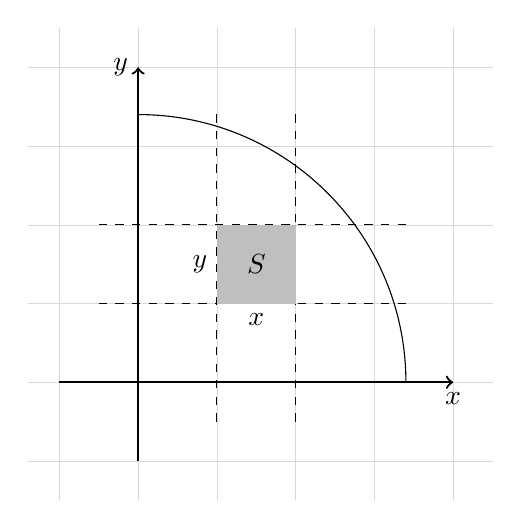
\begin{tikzpicture}
  \draw[very thin, gray!30, step = 1cm] (-1.4, -1.5) grid (4.5, 4.5);
  \draw (3.4, 0) arc (0 : 90 : 3.4cm);

  \draw[thick] [->] (-1, 0) -- (4, 0) node[below] {\(x\)};
  \draw[thick] [->] (0, -1) -- (0, 4) node[below, left] {\(y\)};

  \draw[dashed] (1, -0.5) -- (1, 3.5);
  \draw[dashed] (2, -0.5) -- (2, 3.5);
  \draw[dashed] (-0.5, 1) -- (3.5, 1);
  \draw[dashed] (-0.5, 2) -- (3.5, 2);
  \fill[lightgray] (1, 1) -- (1, 2) -- (2, 2) -- (2, 1) -- cycle;

  \draw node[below] at (1.5, 1) {\(\dd x\)};
  \draw node[left] at (1, 1.5) {\(\dd y\)};
  \draw node at (1.5, 1.5) {\(\dd S\)};
\end{tikzpicture}

    \caption{\(\dd S = \dd x \dd y\)}\label{fig:curve-coords-dcs}

  \end{subfigure}
  \qquad
  \begin{subfigure}[b]{0.4\textwidth}

    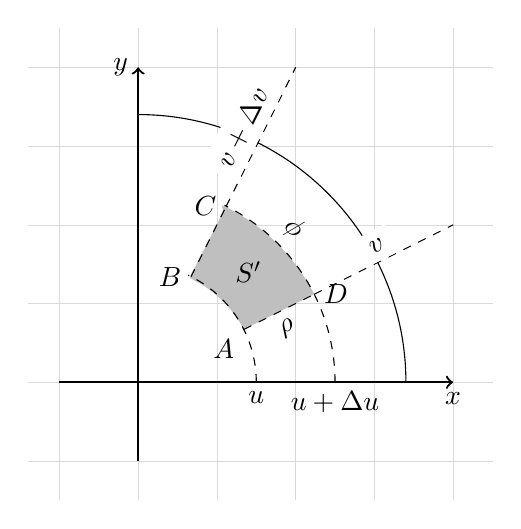
\begin{tikzpicture}
  \draw[very thin, gray!30, step = 1cm] (-1.4, -1.5) grid (4.5, 4.5);
  \draw (3.4, 0) arc (0 : 90 : 3.4cm);

  \draw[thick] [->] (-1, 0) -- (4, 0) node[below] {\(x\)};
  \draw[thick] [->] (0, -1) -- (0, 4) node[below, left] {\(y\)};
  
  %% нет, мне не стыдно
  \fill[lightgray] (1.342, 0.671) arc (28 : 65 : 1.5cm)
    -- (1.118, 2.236)
    -- cycle;
  \fill[lightgray] (2.236, 1.118) arc (27 : 65 : 2.5cm)
    -- (1.342, 0.671)
    -- cycle;

  \draw[dashed] (1.5, 0) arc (0 : 65 : 1.5cm);
  \draw[dashed] (2.5, 0) arc (0 : 64 : 2.5cm)
    node[pos = 0.7, sloped, above] {\(\dd \phi\)};
  \draw[dashed] (0.671, 1.342) -- (1.118, 2.236);
  \draw[dashed] (1.342, 0.671) -- (2.236, 1.118)
    node[midway, sloped, below] {\(\dd \rho\)};

  \draw node[below left] (A) at (1.342, 0.671) {\(A\)};
  \draw node[left] (B) at (0.671, 1.342) {\(B\)};
  \draw node[left] (C) at (1.118, 2.236) {\(C\)};
  \draw node[right] (D) at (2.236, 1.118) {\(D\)};
  \draw node at (1.4, 1.4) {\(\dd S'\)};

  \draw node[below] at(1.5, 0) {\(u\)};
  \draw node[below] at(2.5, 0) {\(u + \Delta u\)};

  \draw[dashed] (2.236, 1.118) -- (4, 2)
    node[fill = white, midway, sloped, above] {\(v\)};
  \draw[dashed] (1.118, 2.236) -- (2, 4)
    node[fill = white, midway, sloped, above] {\(v + \Delta v\)};
\end{tikzpicture}

    \caption{\(\dd S' \neq \dd \rho \dd \phi\)}\label{fig:curve-coords-pcs}

  \end{subfigure}
\end{figure}


Дробление в выбранной СК проводится соответствующими координатными
линиями/поверхностями. Потребуем малости \(\dd u\), \(\dd v\). Тогда площадь
криволинейного прямоугольника будет мало отличать от площади обычного
прямоугольника \(ABCD\), значит:

\begin{align*}\label{eq:curve_coords_det}\tag{1}
  \dd S'
  = \abs{\vec{AB} \times \vec{AD}}
  = \abs{\begin{vmatrix}
    \vec{i} & \vec{j} & \vec{k} \\
    B_{x} - A_{x} & B_{y} - A_{y} & 0 \\
    D_{x} - A_{x} & D_{y} - A_{y} & 0
  \end{vmatrix}}
\end{align*}

Рассмотрим полученные разницы координат точек:

\begin{align*}
  B_{x} - A_{x}
  = \phi(u, v + \Delta v) - \phi(u, v)
  =  \Delta_{v} \phi \approx \frac{\partial \phi}{\partial v} \dd v
  \\
  B_{y} - A_{y}
  = \psi(u, v + \Delta v) - \psi(u, v)
  =  \Delta_{v} \psi \approx \frac{\partial \psi}{\partial v} \dd v
  \\
  D_{x} - A_{x}
  = \phi(u + \Delta u, v) - \phi(u, v)
  =  \Delta_{u} \phi \approx \frac{\partial \phi}{\partial u} \dd u
  \\
  D_{y} - A_{y}
  = \psi(u + \Delta u, v) - \psi(u, v)
  =  \Delta_{u} \psi \approx \frac{\partial \psi}{\partial u} \dd u
\end{align*}

Подставим это в \eqref{eq:curve_coords_det}. Имеем:

\begin{align*}
  \dd S' \approx \abs{ \left(
    \frac{\partial \phi}{\partial v} \dd v \cdot
      \frac{\partial \psi}{\partial u} \dd u 
    -
    \frac{\partial \psi}{\partial v} \dd v \cdot 
    \frac{\partial \phi}{\partial u} \dd u
  \right)}
  = \under{\abs{
    \frac{\partial \phi}{\partial v} \cdot
    \frac{\partial \psi}{\partial u}
    -
    \frac{\partial \psi}{\partial v} \cdot 
    \frac{\partial \phi}{\partial u}
  }}{\abs{J}} \cdot \dd u \dd v
\end{align*}

\(\abs{J}\) можно записать в виде определителя:

\begin{align*}
  \abs{J} = \abs{\begin{vmatrix}
    \phi'_{v} & \phi'_{u} \\
    \psi'_{v} & \psi'_{u}
  \end{vmatrix}}
\end{align*}

\begin{definition}
  Определитель \(J\) составленный из частных производных исходных переменных
  по каждой из новых переменных называется определителем Якоби (якобианом).

  Его геометрический смысл заключается в том, что он является коэффициентом
  искажения при переходе от одной СК к другой.
\end{definition}

В итоге получаем, что \(\dd S = \dd x \dd y = \abs{J} \dd \rho \dd \phi\),
причем \(\displaystyle
  \abs{J}
  = \lim_{\Delta S, \Delta S' \to 0} \frac{\Delta S'}{\Delta S}
\). Итоговая формула замены при смене СК имеет вид:

\begin{align*}
  \iint_{D} f(x, y) \dd x \dd y
  = \iint_{D'} f(x(u, v), y(u, v)) \abs{J} \dd u \dd v
\end{align*}

\begin{remark}
  Якобиан при стандартном переходе в полярные координаты
  (\(x = \rho \cos \phi, y = \rho \sin \phi\)) равен \(\rho\).
\end{remark}

В тройном интеграле замены проводятся аналогично (только якобиан будет третьей
размерности). Некоторые стандартные замены можно найти в предыдущем вопросе.
